\section{Properties of Solutions to the Schrödinger Equation}

\subsection{Real Solutions}\label{real_solutions}

We now take a brief intermission to discuss some general properties of solutions to the Schrödinger equation. First, we can show that $V(x)$ being real allows us to work with real eigenstates.

\begin{framedthm}[Real eigenstates]\label{real_eigenstates}
    The energy eigenstates $\psi(x)$ can be chosen to be real.

    \begin{proof}
        Consider the time-independent Schrödinger equation $$\psi''+\frac{2m}{\hbar^2}(E-V(x))\psi=0.$$Since $(\psi'')^=(\psi^*)''$ and $V(x)$ is real, taking the complex conjugate of the above equation gives $$(\psi^*)''+\frac{2m}{\hbar^2}(E-V(x))\psi^*=0.$$Thus, we see that $\psi^*$ is another solution *with the same energy*. By linearity, we can obtain the real degenerate solutions $$\psi_r=\frac{1}{2}(\psi+\psi^*),\quad\psi_{im}=\frac{1}{2i}(\psi-\psi^*).$$These represent the real and imaginary parts of $\psi$. 
    \end{proof}
\end{framedthm}

Furthermore, if we restrict ourselves to bound states, \textit{all} solutions are real, up to a constant complex phase.

\begin{framedcor}[Real bound states]\label{real_bound_states_cor}

    Any bound state $\psi$ of a one-dimensional potential is real, up to a constant phase.

    \begin{proof} By Theorem \ref{non-degeneracy_of_bound_states}, we know that there are no degenerate bound states in one-dimensional potentials. Thus, the two real solutions $\psi_r$ and $\psi_{im}$ considered above must be equal up to a constant $c\in\mathbb{R}$: $$\psi_{im}(x)=c\psi_r(x).$$It then follows that $\psi=\psi_r+i\psi_{im}=(1+ic)\psi_r$. We can express $1+ic=\sqrt{1+c^2}e^{i\beta}$, which shows that $\psi$ is real up to the constant phase $\beta$. \end{proof}
\end{framedcor}

\subsection{Even Potentials}\label{even_potentials}

Suppose the potential $V(x)$ is even --- that is, it satisfies $V(-x)=V(x)$ for all $x$. It turns out that we can then work with only even and odd wavefunctions.

\begin{framedthm}[Even potentials]\label{even_potential_thm}
    If $V(-x)=V(x)$, the energy eigenstates can be chosen to all be even or odd.

    \begin{proof} Again, we begin with the time-independent Schrödinger equation $$\psi''(x)+\frac{2m}{\hbar^2}(E-V(x))\psi(x)=0.$$We can substitute $-x$ for $x$ to get $$\psi''(-x)+\frac{2m}{\hbar^2}(E-V(x))\psi(-x)=0,$$where we used the fact that $V(x)$ is even. We wish to show that the above equation implies that $\psi(-x)$ is another solution of the Schrödinger equation with the same energy. We define a function $\phi(x)\equiv\psi(-x)$. We see that $$\phi'(x)=-\psi'(x), \text{ and  }\,\phi''(x)=\psi''(-x).$$Thus we have $$\phi''(x)+\frac{2m}{\hbar^2}(E-V(x))\phi(x)=0.$$Therefore, $\phi(x)=\psi(-x)$ is a degenerate solution with the same energy as $\psi$. We can now form the symmetric and antisymmetric combinations $$\psi_s(x)=\frac{1}{2}(\psi(x)+\psi(-x)),\quad\psi_a(x)=\frac{1}{2}(\psi(x)-\psi(-x)).$$These solutions are even and odd, respectively. \end{proof}
\end{framedthm}

Again, if we restrict ourselves to bound states of one-dimensional even potentials, \textit{all} solutions are even or odd.

\begin{framedcor}[Bound states of even potentials]\label{even_potential_cor}
    Any bound state $\psi$ of a one-dimensional even potential is either even or odd.

    \begin{proof}
        Recall from Theorem \ref{non-degeneracy_of_bound_states} that there are no degenerate bound states in one-dimensional potentials. By Corollary \ref{real_bound_states_cor}, $\psi$ is real up to a constant phase, so we must have $$\psi(-x)=c\psi(x)$$for some real constant $c$. Letting $x\rightarrow -x$, we have $\psi(x)=c\psi(-x)=c^2\psi(x)$ from which we see that $c^2=1$. The only possibilities are $c=\pm 1$, so $\psi(x)$ must be even or odd.
    \end{proof}
\end{framedcor}

This result is why we restricted ourselves in Section \ref{finite_square_well} to even and odd bound states. The finite square well is symmetric, and thus cannot have other bound states!

\subsection{The Node Theorem}\label{node_theorem_section}

In Section \ref{nodes_and_symmetries_infinite_square_well}, we noted that the $n$th bound state had $n-1$ nodes. This result is true in general.

\begin{framedthm}[Node theorem]\label{node_thm}
    Given any one-dimensional potential $V(x)$ with bound states $\psi_1,\psi_2,\psi_3,\ldots$ and energy levels $E_1,E_2,E_3,\ldots$, it holds that $\psi_n$ has $(n-1)$ nodes. 
\end{framedthm}

We have seen that Theorem \ref{node_thm} is true for the infinite square well. We now provide an intuitive argument that it holds for any smooth potential $V(x)$ that goes to infinity as $|x|\to\infty$.

Consider an arbitrary such potential. We fix the location $x=0$ at a minimum and define the \textbf{screened potentials} $V_a(x)$ as follows: for any positive real value $a$, we define $$V_a(x)=\begin{cases}V(x)&|x|<a\\\infty&|x|>a \end{cases}$$As shown in Figure \ref{screened}, $V_a(x)$ is an infinite well of width $2a$ whose bottom is $V(x)$.

\begin{figure}
    \centering
    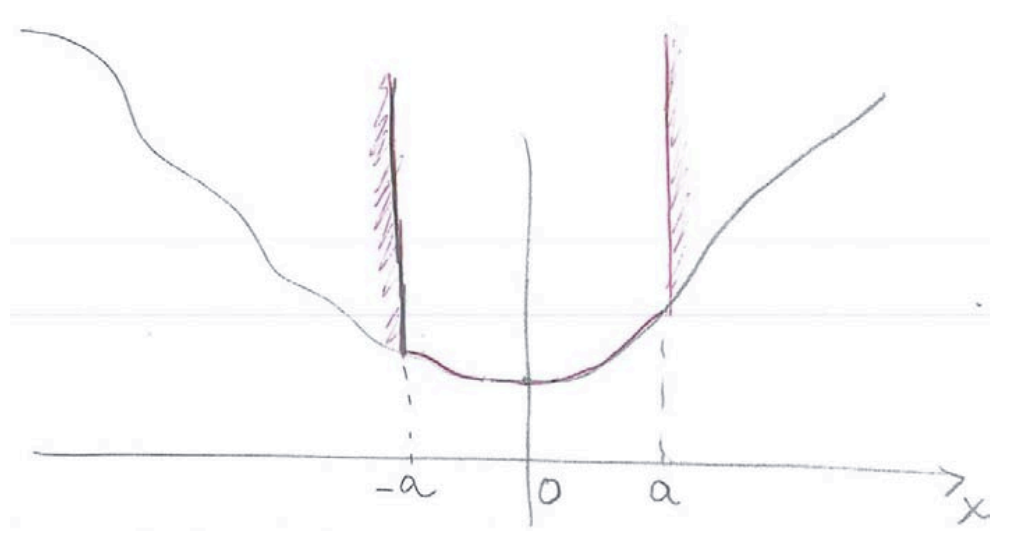
\includegraphics[width=0.5\linewidth]{resources/images/screened.png}
    \caption{The screened potential $V_a(x)$.}
    \label{screened}
\end{figure}

We now take two plausible assumptions. First, as $a$ goes to $\infty$, the bound states of $V_a(x)$ are the bound states of $V(x)$. Additionally, as $a$ increases, the bound states vary continuously.

When $a$ is sufficiently small, $V_a(x)$ can be approximated as a very narrow infinite square well, since we chose $x=0$ to be a minimum and any minimum is locally flat. We know that Theorem \ref{node_thm} holds for this infinite square well. For example, the ground state $\psi$. will have no nodes. We now argue that as $a$ increases, $\psi$ cannot obtain a new node. This argument also holds for all other states.

Suppose a new node is created at $x=a'$ in the potential $V_{a'}(x)$ --- that is, at a boundary of the infinite well. For this to happen, we must have $\psi'(a')>0$, while $\psi'(a)<0$ sufficiently small $a$, as shown in Figure \ref{moving_endpoint}. Assuming continuity, there must be some intermediate screened potential at which $\psi'=0$ at the right endpoint. However, the right endpoint is always the boundary of an infinite well, so $\psi=0$ there. Then we would have $\psi=\psi'=0$ at a point, which would imply that $\psi(x)=0$ for all $x$. This is impossible, so no new nodes can be formed at the boundaries of the well.

\begin{figure}[H]
    \centering
    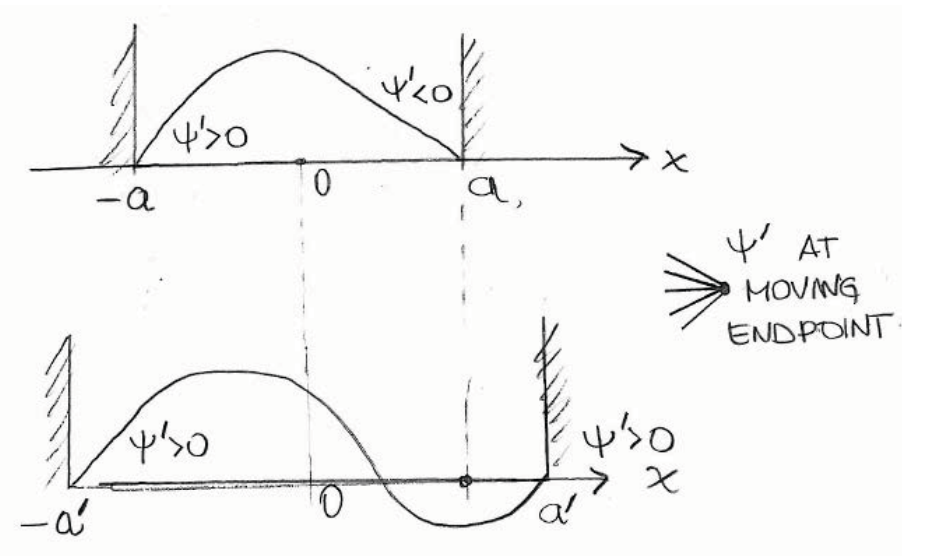
\includegraphics[width=0.5\linewidth]{resources/images/moving_endpoint.png}
    \caption{For sufficiently small $a$, $\psi'(a)<0$. If there exists some $a'$ such that $\psi'(a')>0$, at some point we must have $\psi'=\psi=0$ at the boundary of the well.}
    \label{moving_endpoint}
\end{figure}

We can also imagine introducing a new node at some intermediate point inside the well, so that the sign of $\psi'$ at the endpoints does not change. In this process, shown in Figure \ref{dipping_intermediate}, the wavefunction $\psi$ dips and produces two new nodes. However, this again forces $\psi$ to be tangent to the $x$-axis for some intermediate screen, which is impossible.

\begin{figure}
    \centering
    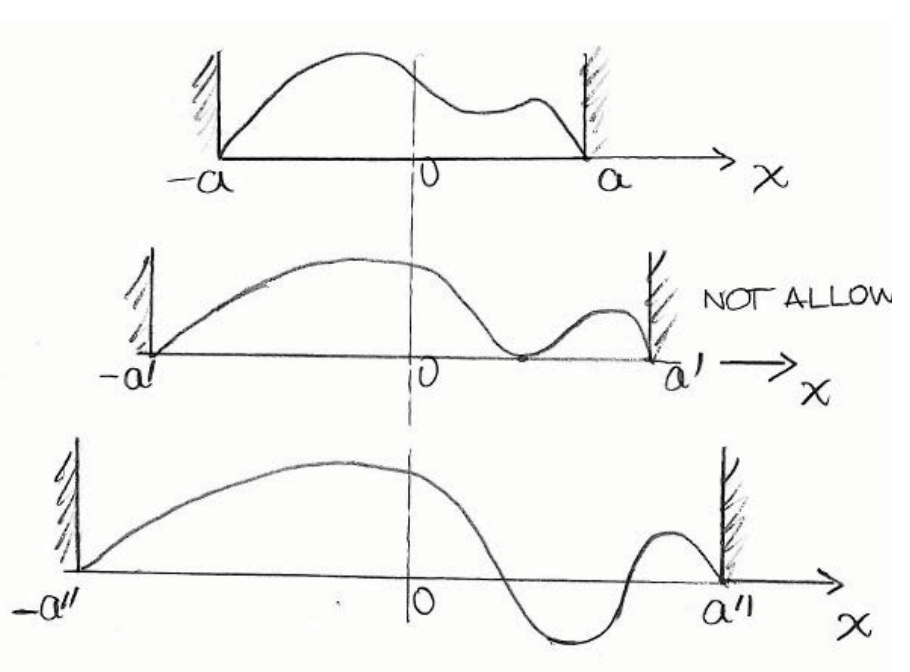
\includegraphics[width=0.5\linewidth]{resources/images/dipping_intermediate.png}
    \caption{If $\psi$ dips below the $x$-axis, there must be an intermediate screen where $\psi$ is tangent to the $x$-axis.}
    \label{dipping_intermediate}
\end{figure}

Since the number of nodes of a wavefunction is constant for all the $V_a(x)$, it must also be the same for $V(x)$. Thus, the node theorem holds for any smooth diverging one-dimensional potential.

\section{The Semi-Classical Approximation}

\subsection{Local de Broglie Wavelength}\label{local_de_broglie}

We will now consider some qualitative insights that classical physics can give us about the behavior of quantum stationary states. This way of thinking is called the \textbf{semi-classical approximation}.

We begin with an example we already understand. Consider the total energy $E$ of a particle as the sum of its potential energy $V$ and its kinetic energy $K$. In our first example, shown in Figure \ref{constant_V}, $V$ is constant. Since $E$ is conserved, $K$ must also be constant. The particle will thus have a constant momentum $p=\sqrt{2mK}$. From Section \ref{deBroglie_proposal}, we know that the wave representing the particle has a de Broglie wavelength $\lambda=\frac{h}{p}$. Indeed, the Schrödinger equation gives $$\psi''=-\frac{2m}{\hbar^2}(E-V)\psi=-\frac{2mK}{\hbar^2}\psi=-\frac{p^2}{\hbar^2}\psi,$$leading to real solutions of the form $$\psi\sim\cos(\frac{p}{\hbar}x)=\cos(\frac{2\pi}{\lambda}x).$$

\begin{figure}
    \centering
    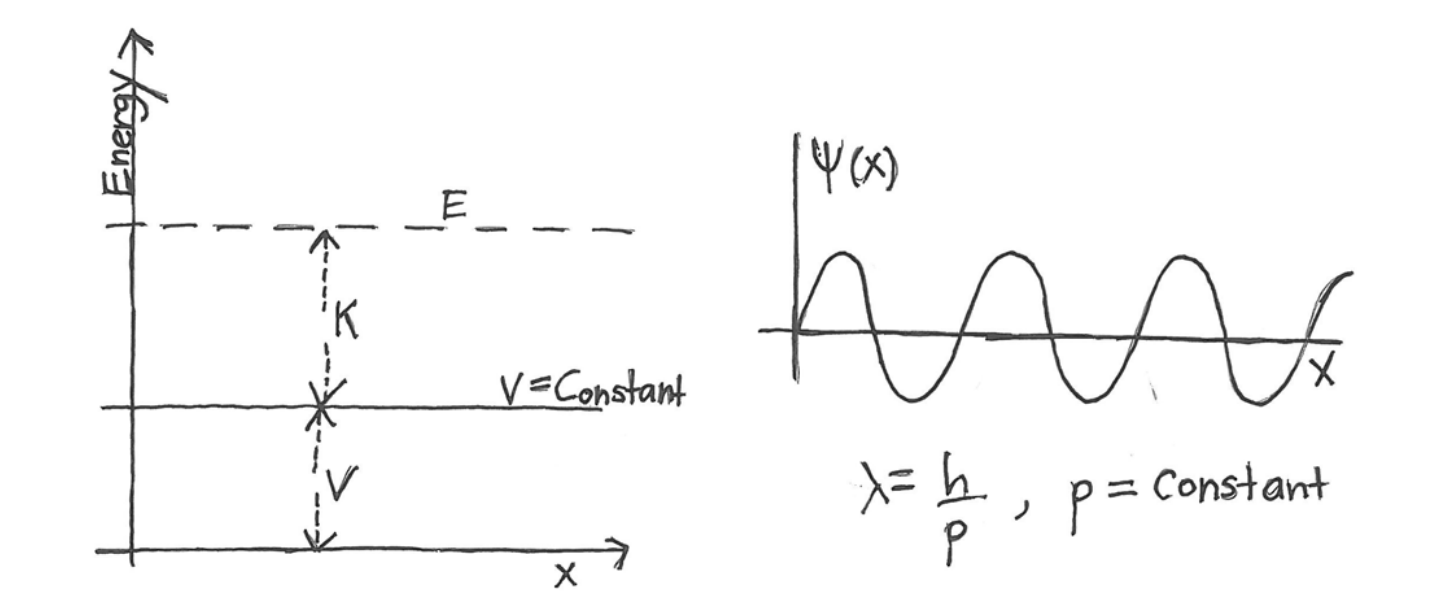
\includegraphics[width=0.5\linewidth]{resources/images/constant_V.png}
    \caption{If $V$ is constant, the particle has constant de Broglie wavelength.}
    \label{constant_V}
\end{figure}

This wavefunction is real and is not a momentum eigenstate; instead, it represents a superposition of a state with momentum $p$ and a state of momentum $-p$. This shouldn't be too surprising; even in the classical case, the kinetic energy only determines $p^2$, and not the sign of $p$.

Consider now the situation depicted in Figure \ref{linearly_increasing_potential}, where we imagine a classical particle moving in a linearly increasing potential $V(x)$. Then the kinetic energy $K(x)$ is also position dependent, and thus so is the momentum $p(x)=\sqrt{2mK(x)}$. As long as the potential is slowly varying, the wavefunction will have a position-dependent de Broglie wavelength approximated by $$\lambda(x)=\frac{h}{p(x)}.$$

\begin{figure}
    \centering
    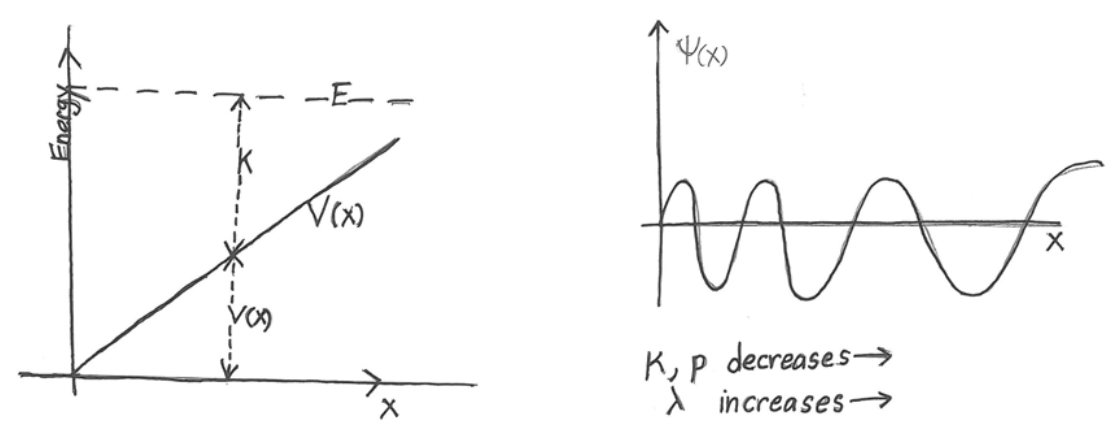
\includegraphics[width=0.5\linewidth]{resources/images/linearly_increasing_potential.png}
    \caption{If $V$ increases, the particle has increasing de Broglie wavelength.}
    \label{linearly_increasing_potential}
\end{figure}

By this we mean that $\psi$ is some combination of functions $$\cos(\frac{2\pi x}{\lambda(x)}),\quad\sin(\frac{2\pi x}{\lambda(x)}).$$This approximation is accurate when the potential changes slowly --- that is, when the change in potential over a distance comparable to the local de Broglie wavelength is very small compared to the potential: $$\lambda(x)\bigg|\frac{dV}{dx}\bigg|\ll |V(x)|.$$

We now draw an arbitrary potential $V(x)$ and consider the classical motion of a particle of total energy $E$. For any point $x_0$, we have $V(x_0)+K(x_0)=E$. The maximum kinetic energy occurs at the minimum value of the potential. The \textbf{forbidden regions} are the regions in which $V(x)>E$, preventing the particle from accessing them. Points where $V(x)=E$ are known as \textbf{turning points}, because the particle must reverse direction at these points.

\begin{figure}
    \centering
    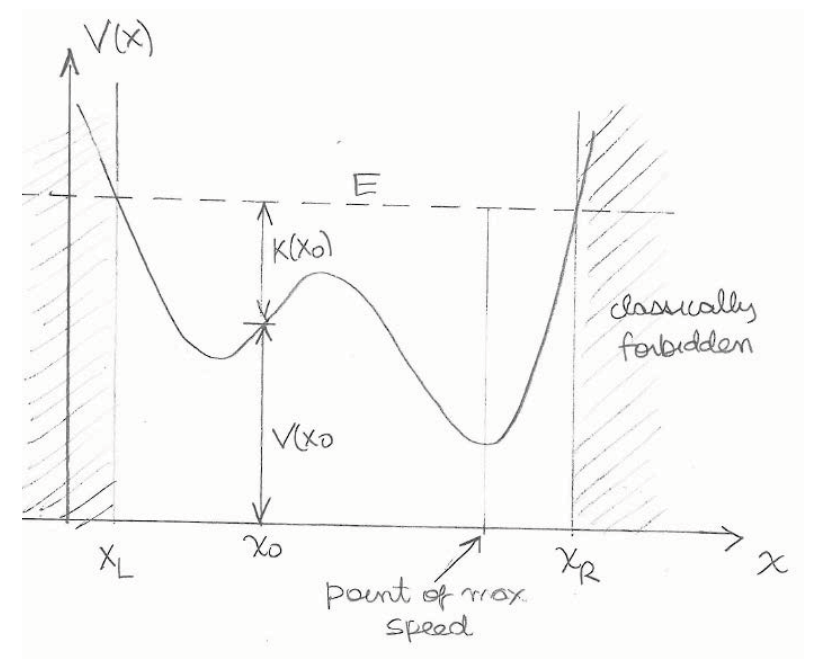
\includegraphics[width=0.5\linewidth]{resources/images/classically_forbidden.png}
    \caption{In the classically forbidden regions, the potential $V(x)$ exceeds the energy $E$ of the particle.}
    \label{classically_forbidden}
\end{figure}

\subsection{The Correspondence Principle}\label{correspondence_principle}

Intuitively, there should be a higher probability of finding the particle in regions where it spends more time. This has significant implications for quantum mechanics.

We already know that the particle is found in a region $dx$ with probability $|\psi|^2dx$. This should also be the fraction of time $\frac{dt}{T}$ that the particle spends in the region. With $v(x)$ the local velocity of the particle, we have that $$|\psi|^2dx\sim\frac{dx}{v(x)T}=\frac{m}{T}\frac{1}{p(x)}dx,$$which implies that the amplitude of the wavefunction is proportional to the square root of the local de Broglie wavelength.

For the linearly increasing potential from Figure \ref{linearly_increasing_potential}, the de Broglie wavelength increases with $x$, so both the amplitude and wavelength of $\psi$ increase with $x$.

\begin{figure}
    \centering
    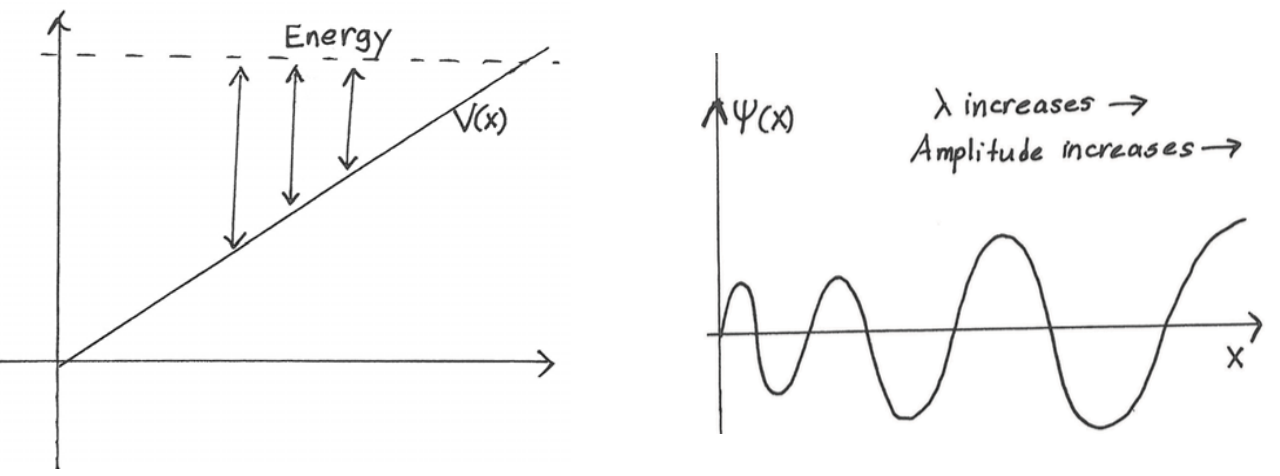
\includegraphics[width=0.5\linewidth]{resources/images/amplitude_increasing.png}
    \caption{In an increasing potential, both the wavelength and amplitude of $\psi$ are increasing.}
    \label{amplitude_increasing}
\end{figure}

For bound states with large energies, averaging $|\psi|$ can be useful to obtain results from classical mechanics. For example, the probability distribution of a particle in an infinite well approaches the classical version when the particle has a very large energy. The idea that there are classical limits of quantum states is called the \textbf{correspondence principle}.

\section{Qualitative Behavior of the Wavefunction}
\subsection{Local Picture of the Wavefunction}\label{local_picture_wavefunction}

From the Schrödinger equation, we have $$\frac{1}{\psi}\frac{d^2\psi}{dx^2}=-\frac{2m}{\hbar^2}(E-V(x)).$$There are three cases for the local behavior of $\psi$.

\begin{enumerate}
    \item The \textbf{classically forbidden region} $E-V(x)<0$. Then the right-hand side of the Schrödinger equation is positive, so either $\psi$ and $\psi''$ are both positive or they are both negative. These possible behaviors are summarized by saying that the wavefunction is \textit{convex towards the axis}. When classically forbidden regions reach to $x=\pm\infty$, the behavior looks like the first sketch in Figure \ref{local_picture}.
    \item The \textbf{classically allowed region} $E-V(x)>0$. Then the right-hand side of the Schrödinger equation is negative, so either $\psi$ is positive and $\psi''$ is negative, or vice versa. This can be summarized by saying that the wavefunction is \textit{concave towards the axis}, as shown in the second skect in Figure \ref{local_picture}. A large classically allowed region has $\psi$ alternating positive and negative, creating a function resembling a sinusoid.
    \item The \textbf{turning points} $E-V(x)=0$. Then we have $\frac{1}{\psi}\psi''=0$, so the turning points are \textit{inflection points} in the graph of $\psi(x)$. Note that not all inflection points are turning points -- in fact, all nodes of the wavefunction are inflection points, since $\psi''=-\frac{2m}{\hbar^2}(E-V(x))\psi=0$ when $\psi(x)=0$. 
\end{enumerate}

\begin{figure}
    \centering
    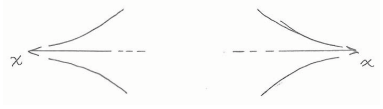
\includegraphics[width=0.4\linewidth]{resources/images/convex.png}
    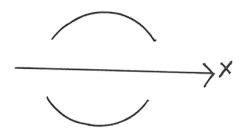
\includegraphics[width=0.4\linewidth]{resources/images/concave.png}
    \caption{When $E-V<0$, the wavefunction looks like the left sketch. When $E-V>0$, the wavefunction looks like the right sketch.}
    \label{local_picture}
\end{figure}

\subsection{Energy Eigenstates on a Generic Symmetric Potential}\label{energy_eigenstates_on_generic_symmetric_potential}

The first sketch in the following diagram displays a smooth, symmetric potential $V(x)$. We wish to see qualitatively why the possible energy levels of bound states in this potential are discrete. The classically forbidden regions must contain $x=\pm\infty$. Without loss of generality, we assume that the end behavior of $\psi$ is positive as $x\rightarrow\infty$, as shown in the top right of Figure \ref{generic_eigenstate}.

\begin{figure}
    \centering
    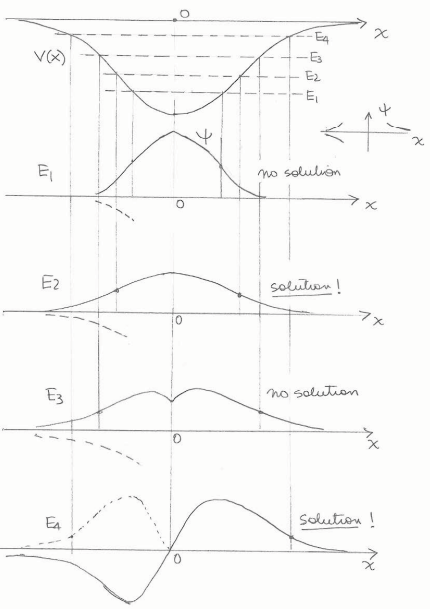
\includegraphics[width=0.7\linewidth]{resources/images/generic_eigenstate.png}
    \caption{Integrating the Schrödinger equation for four energy levels.}
    \label{generic_eigenstate}
\end{figure}

As shown above, we consider the four energies $E_1<E_2<E_3<E_4$, where not all correspond to eigenstates. We imagine integrating the Schrödinger equation from $x=\infty$ to $x=0$ for each value of $E$. 

For example, consider integrating for $E=E_1$. Coming in from $x=\infty$, the solution has an inflection point and becomes concave towards the axis. The same thing happens when coming in from $x=-\infty$. However, the two segments do not match at $x=0$; $\psi'$ fails to be continuous. Thus, $E_1$ is not an allowed energy.

As we increase the energy to $E=E_2$, the turning point occurs for larger and larger $x$, and $\psi'(0)$ is eventually exactly $0$ at $E=E_2$. This represents the ground state of the potential, which is an even solution.

Continuing to increase the energy to $E=E_3$, the turning point becomes even farther away from $x=0$, and $\psi'(0)$ becomes negative. This again cannot be a solution, since $\psi'$ is discontinuous at $x=0$.

Finally, increasing the energy further to some value $E_4$ allows $\psi(0)$ to be exactly $0$. As shown, we can match this to an odd solution. This represents the first excited state of the potential, with a single node at $x=0$.

\subsection{The Shooting Method}\label{shooting_method}

The \textbf{shooting method} is a numerical method to find the form of bound solutions $\psi$ for even potentials $V(x)$. 

We first consider even states. We pick some arbitrary energy $E_0$, and we choose $\psi(0)=1$ since we ignore normalization constants. We must also have $\psi'(0)=0$, since $\psi$ is continuous and even. 

We proceed by integrating the Schrödinger equation numerically. Most likely, $E_0$ will not be an allowed energy value. This will manifest in $\psi$ diverging beyond some value of $x$. Suppose $\psi\rightarrow\infty$. Then we must change the value of the energy until we find some value $E_1$ for which the solution also diverges, but this time with $\psi\rightarrow-\infty$. This is a sign that there is some energy \textit{in between} $E_0$ and $E_1$ for which $\psi$ is normalizable. We then try to narrow this interval, obtaining increasingly better approximations for the actual bound-state energy.

For odd solutions, the procedure is the same, but this time the boundary conditions are $\psi(0)=0$ and $\psi'(0)=1$. The first condition is a requirement for $\psi$ to be odd and continuous, and the second is arbitrary up to normalization.

\begin{framedrmk*}[A practical note]
    When working with computers to carry out these numerical integrations, it is first necessary to clean out the units from the differential equation. That is, we must replace $x$ with a unit-free variable $u$ such that $x=bu$, for some quantity $b$ with units of length built from the parameters in the problem.
\end{framedrmk*}

\section{The Delta Function Potential}

\subsection{Setting Up the Delta Function Potential}\label{setting_up_delta_function}

The \textbf{delta function potential} is an important application of Theorem \ref{node_thm} and the qualitative pictures in Section \ref{energy_eigenstates_on_generic_symmetric_potential}. We consider a particle of mass $m$ moving in the one-dimensional potential $$V(x)=-\alpha\delta(x),$$where $\alpha$ is a positive constant. This potential is shown in Figure \ref{delta_potential_graph}, where the delta function is represented by a downward arrow.

\begin{figure}
    \centering
    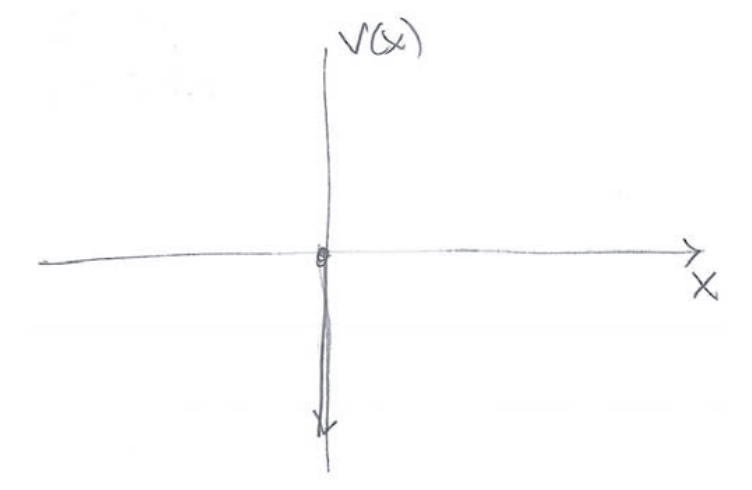
\includegraphics[width=0.5\linewidth]{resources/images/delta_potential.png}
    \caption{A graph of the delta function potential.}
    \label{delta_potential_graph}
\end{figure}

We want to know if this potential admits bound states -- that is, states with energy $E<0$. We gain some intuition by considering units. The dimension-full constants in the problem are $\alpha$, $m$, and $\hbar$. Since a delta function has units of $\frac{1}{L}$, the constant $\alpha$ must have units of energy times length. By dimensional analysis, we see that $$[E]=[\frac{m\alpha^2}{\hbar^2}].$$Therefore, the energy $E_b$ of any bound state must be a negative number times this value: $$E_b=-u\frac{m\alpha^2}{\hbar^2}.$$To find the ground state energy, we only need to find a unit-free number $u$, which we can guess is of order $u \approx 1$.

We can gain further intuition by trying to draw the ground state wavefunction. We can approximate the delta function as a finite square well in the limit of the width going to 0 and the depth going to infinity. As shown in Figure \ref{finite_square_well_limit}, the width of the well provides the curvature needed for the wavefunction to have a continuous derivative. In the limit of an infinitely thin well, the derivative becomes discontinuous at $x=0$.

We now consider the relevant differential equations given by the time-independent Schrödinger equation. For $x\neq 0$, we have $$\psi''=-\frac{2mE}{\hbar^2}\psi=\kappa^2\psi,$$where $\kappa^2=-\frac{2mE}{\hbar^2}>0$. The solutions are of the form $$e^{\kappa x},\,e^{-\kappa x}.$$

\begin{figure}[H]
    \centering
    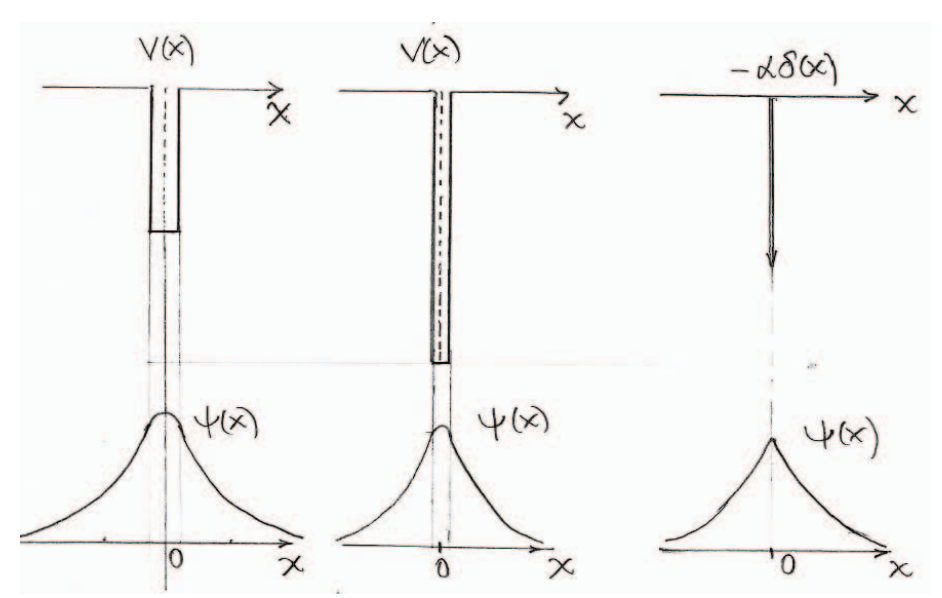
\includegraphics[width=0.5\linewidth]{resources/images/limit_finite_square_wells.png}
    \caption{The delta function potential can be thought of as a finite square well in the limit of width going to $0$ and depth going to $\infty$.}
    \label{finite_square_well_limit}
\end{figure}

Note that the potential is even, so the ground state must be even and have no nodes. The first excited state must then be odd and have a node at $x=0$. However, the only odd solution we can build with the above exponentials is proportional to $$\sinh(\kappa x)\sim e^{\kappa x}-e^{-\kappa x}.$$However, a wavefunction $\psi\sim\sinh(\kappa x)$ certainly cannot be normalized, since it diverges at $x=\pm\infty$. Therefore, there cannot be an excited state in the delta function potential. Without solving anything, we know that if there are bound states, there is just one!

\subsection{Solving the Delta Function Potential}\label{solving_the_delta_potential}

For $\psi$ to be normalizable and continuous, we must have $\psi(x)=Ae^{-\kappa x}$ for $x>0$, and $\psi(x)=Ae^{\kappa x}$ for $x<0$. Thus, the solution must be of the form $$\psi(x)=Ae^{-\kappa|x|}.$$To constrain the possible values of $\kappa$, we rewrite the Schrödinger equation: $$-\frac{\hbar^2}{2m}\psi''+V(x)\psi=E\psi.$$We integrate this equation from $-\epsilon$ to $\epsilon$, with $0<\epsilon\ll 1$, a range that includes the entirety of the delta function. This gives $$-\frac{\hbar^2}{2m}(\frac{d\psi}{dx}\bigg|_\epsilon-\frac{d\psi}{dx}\bigg|_{-\epsilon})+\int_{-\epsilon}^\epsilon dx\,(-\alpha\delta(x))\psi(x)=E\int_{-\epsilon}^\epsilon \psi(x)\,dx.$$In the limit as $\epsilon$ goes to $0$, the integral on the right-hand side vanishes because $\psi(x)$ is finite for all $x$. Meanwhile, the integral of the delta function times $\psi(x)$ simply evaluates $\psi$ at $x=0$, so we have $$-\frac{\hbar^2}{2m}\lim_{\epsilon\to 0}\,(\frac{d\psi}{dx}\bigg|_\epsilon-\frac{d\psi}{dx}\bigg|_{-\epsilon})-\alpha\psi(0)=0.$$We define the \textbf{discontinuity} of $\psi'$ as follows.

\begin{frameddefn}[Discontinuity]
    The \textbf{discontinuity} $\Delta_0$ of $\psi'$ at $x=0$ is $$\Delta_0(\psi')=\lim_{\epsilon\to 0}\,(\frac{d\psi}{dx}\bigg|_\epsilon-\frac{d\psi}{dx}\bigg|_{-\epsilon}).$$As its name suggests, it represents the difference between the slope of the wavefunction just to the right of $x=0$ and just to the left of $x=0$.
\end{frameddefn}

We have now learned that $$\Delta_0(\psi')=-\frac{2m\alpha}{\hbar^2}\psi(0).$$Applying this relation to our solution $\psi(x)=Ae^{-\kappa|x|}$, we have $$\lim_{\epsilon\to 0}(-\kappa Ae^{-\kappa\epsilon}-\kappa Ae^{-\kappa\epsilon})=-2\kappa A=-\frac{2m\alpha}{\hbar^2}A.$$This relation fixes the value of $\kappa$: $$\kappa=\frac{m\alpha}{\hbar^2}.$$Therefore, the bound state energy is $$\boxed{E_b=-\frac{\hbar^2\kappa^2}{2m}=-\frac{1}{2}\frac{m\alpha^2}{\hbar^2}}.$$As we anticipated by dimensional analysis, the answer is proportional to $\frac{m\alpha^2}{\hbar^2}$. The proportionality constant $u$ turns out to be $\frac{1}{2}$.